% \vspace{-6mm}
\section{Hallucination: The What and Why}
% {What is a hallucination? Why is it alarming?}

\vspace{-4mm}
\begin{figure}[!ht]
    \centering
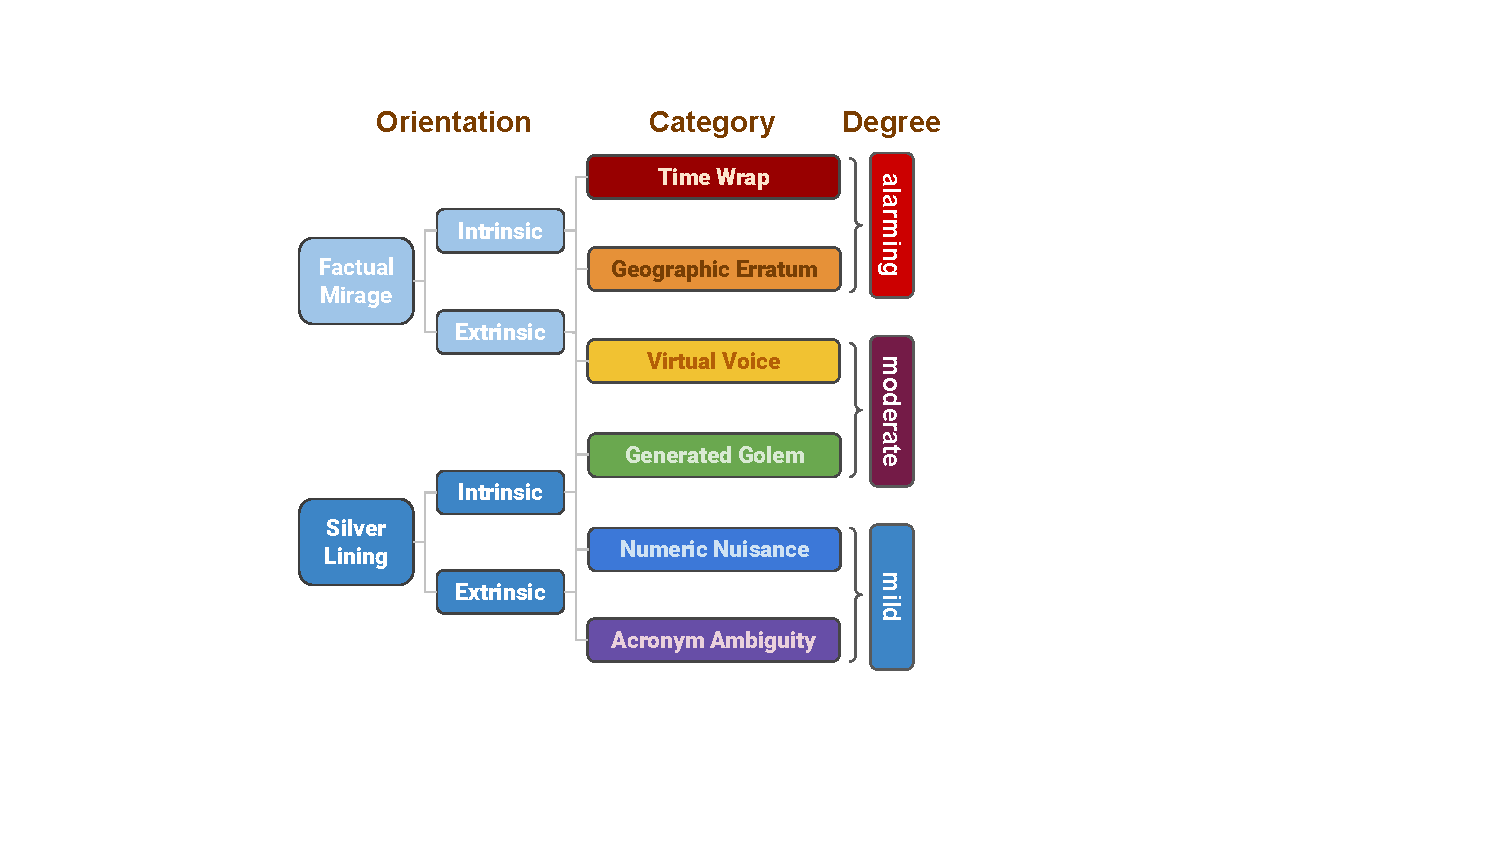
\includegraphics[width=7cm,height=6cm]{img/types.pdf}
\vspace{-2mm}
\caption{Hallucination: orientation,  category, and degree (decreasing level of difficulty from top to bottom).}
%-- red to violet).}
    \label{fig:types}
\end{figure}
\vspace{-2mm}

\noindent
The extraordinary benefits of large generative AI models such as GPT \citep{brown2020language,openai2023gpt4}, Stable Diffusion \cite{rombach2022high}, DALL-E \cite{ramesh2021zero,ramesh2022hierarchical}, and Midjourney \cite{midjourney} also come with a substantial risk of misuse. The alarm this has triggered is reflected in the open letter \cite{aihalt2023} in March 2023 by thousands of researchers and tech leaders calling for a six-month moratorium on training AI systems that are more sophisticated than GPT-4. The key underlying concern is ``\textit{\ul{should we let machines flood our information channels with propaganda and untruth?}}''. In fact, the majority of these falsehoods are widely recognized as \textit{hallucination}, which can be defined as \textit{the generation of content that deviates from the real facts, resulting in unfaithful outputs \cite{maynez-etal-2020-faithfulness}}. 
%\cref{tab:hallucination_ex} presents two instances of hallucination generated by LLMs. 

To address the inevitable question of ownership attribution for AI-generated artifacts, the US Copyright Office  \cite{copyright_2023} released a statement stating that \ul{if the content is traditional elements of authorship produced by a machine, the work lacks human authorship and the office will not register it for copyright}. 
OpenAI's response to the prevalent societal pressure led them to issue a public statement \cite{openaisafety} emphasizing their commitment to AI safety and their determination to implement improved controls on hallucination in future iterations of GPT. The recent roll-out of Google's highly anticipated ChatGPT rival, Bard, led to a fiasco owing to it hallucinating a factually inaccurate answer in the company's advertisement, which cost Google a \$140 billion wipeout in terms of market value \cite{goog}. In the ad, Bard is prompted: \emph{What new discoveries from the James Webb Space Telescope (JWST)...} Bard responds with a number of answers, including one suggesting the \emph{JWST was used to take the very first pictures of a planet outside the Earth's solar system...}. The first pictures of exoplanets were, however, taken by the European Southern Observatory's VLT in 2004. In another incident, a lawyer used ChatGPT to help him prepare a filing in a lawsuit against a US airline. However, ChatGPT quoted a fabricated previous case precedent, which led the judge to consider imposing sanctions \cite{forbes2023}.
%Yet another incident Steven Schwartz, a lawyer filed a case in the USA suing an airline used ChatGPT to prepare a filing, but the LLM delivered fake cases that the attorney then presented to the court, prompting a judge to weigh sanctions.
Amidst these happenings, NVIDIA introduced \textit{NeMo Guardrails} \cite{nemo}, an open-source toolkit, based on the Self-Check GPT framework \cite{manakul2023selfcheckgpt}, designed to address hallucinations in conversational AI systems. 

The remarkable capabilities of generative AI have undeniably propelled it to a superpower status! Although the term \emph{hallucination} has gained widespread acceptance in describing the irrational and uncontrolled behaviors of LLMs, it is important to note that many experts expressed dissatisfaction with this particular nomenclature.  Within the AI community, efforts persist to find a more suitable alternative name to describe this phenomenon accurately. During an interview \cite{YouTube_2023}, Prof. Christopher Manning 
% from Stanford University 
briefly expressed his discontent with the term ``hallucination'', indicating a preference for an alternative term. In the ongoing conversation, Prof. Gary Marcus has advocated for a reframing of ``hallucination'' as \emph{confabulation}, a term that some fellow researchers have already embraced. However, in this paper, we have decided to uphold the use of the term ``hallucination''. In order to offer a comprehensive and precise description of the various types of hallucinations, we will introduce a few new terms. These newly introduced monikers aim to accurately capture and articulate the different categories of hallucinations. 
%discussed in this paper.

%\adt{we need a paragraph saying no previous research take a holistic approach to hallucination - cite all the related previous works}

Contrary to the common belief that hallucinations are negative, certain researchers \cite{cao2022hallucinated} propose that hallucinations in LLMs could have positive implications for text summarization. The authors argue that in certain cases, factual hallucinations can be advantageous in a summary by offering valuable background information. 
% With the widespread adoption of LLMs in a plethora of real-world use cases, it is essential to continue studying the potential benefits and drawbacks of LLM-generated outputs to fully understand their impact in different contexts. 
Furthermore, both the United States \cite{whitehouseaibill} and the European Union \cite{euaiproposal} governments have recently drafted their initial proposals regarding the regulatory framework for AI. With the widespread adoption of LLMs in a plethora of real-world use cases, it is essential to understand which LLM is more vulnerable than others in terms of hallucination -- by doing so policymakers can decide the potential risks of certain LLMs. To this end, we introduce a quantifiable spectrum -- \emph{Hallucination Vulnerability Index (HVI)}, which facilitates the evaluation and ranking of LLMs according to their hallucination vulnerability levels.

\vspace{-2mm}
%\begin{strip}
%\begin{tcolorbox}
%[colback=blue!5!white,colframe=blue!75!black,title=\textbf{\footnotesize \ul{\textsc{Our Contributions}}:} {\footnotesize 
% [left=9pt,right=2pt,colback=Brown!5!white,colframe=Brown!75!black,title={ \footnotesize \fontfamily{qbk} \selectfont \textbf{\ul{Our Contributions}}}: {\footnotesize 
%Deciphering the spectrum of hallucination over a range of LLMs based on HVI.}]
\begin{tcolorbox}[left=9pt,right=2pt,colback=Brown!5!white,colframe=Brown!75!black,title={ \footnotesize \fontfamily{qbk} \selectfont \textbf{\ul{Our Contributions}}}: {\footnotesize \textbf{Deciphering the spectrum of hallucination over a range of LLMs based on HVI}}]
% proposing Hallucination Vulnerability Index (HVI)}]
% - pertaining questions]
\vspace{-2mm}
\begin{itemize}
\setlength\itemsep{0em}
\begin{spacing}{0.85}
\item[\ding{224}] 
{\footnotesize 
{\fontfamily{phv}\fontsize{8}{9}
%\begin{spacing}{1}
\selectfont
Presenting a detailed study to unveil how different (15) LLMs hallucinate when given a \textit{\ul{factually correct prompt}} vs. a \textit{\ul{factually incorrect prompt}}. We name them as \emph{factual mirage} and \emph{silver lining} -- each sub-categorized into \emph{intrinsic} and \emph{extrinsic}, with three degrees of severity: (a) \emph{mild}, (b) \emph{moderate}, and (c) \emph{alarming} (cf. \cref{sec:cat_hallucination})}.
%\end{spacing}
}

\item[\ding{224}] 
{\footnotesize 
{\fontfamily{phv}\fontsize{8}{9}\selectfont
Meticulously categorizing hallucination into \textbf{six} types: (a) \emph{acronym ambiguity}, (b) \emph{numeric nuisance}, (c) \emph{generated golem}, (d) \emph{virtual voice}, (e) \emph{geographic erratum}, and (f) \emph{time wrap} (cf. \cref{sec:cat_hallucination})}.
}

\item[\ding{224}] 
{\footnotesize 
{\fontfamily{phv}\fontsize{8}{9}\selectfont
Introducing 
\includegraphics[height=0.2cm,width=0.9cm]{img/hilt.png} (\textbf{H}alluc\textbf{I}nation e\textbf{L}ici\textbf{T}ation), a publicly available dataset comprising of \ul{75,000} text snippets generated using 
% curated prompts fed to 
15 contemporary LLMs along with human annotations for the aforementioned categories (cf. \cref{sec:hilt_dataset})}.
}

\item[\ding{224}] 
{\footnotesize 
{\fontfamily{phv}\fontsize{8}{9}\selectfont
Introducing \textbf{HVI} (\emph{\ul{Hallucination Vulnerability Index)}} to perform a quantitative analysis of the inclination of various LLMs to hallucination. (cf. \cref{sec:hvi})}. HVI characterizes LLMs based on the proposed types of hallucination vulnerabilities (cf. \cref{fig:hvi-cat}).}

\begin{comment}
\item[\ding{224}] 
{\footnotesize 
{\fontfamily{phv}\fontsize{8}{9}\selectfont
Characterizing LLMs based on the proposed types of hallucination vulnerabilities (cf. \cref{sec:behaviors_hvi})}.
}
\end{comment}

\item[\ding{224}] 
{\footnotesize 
{\fontfamily{phv}\fontsize{8}{9}\selectfont
While complete mitigation can be a herculean task, we suggest 2 mitigation strategies to alleviate hallucination. We propose to identify high-entropy points in text generated by an LLM with a high HVI and replace them using an LLM with a lower HVI, yielding desired results (cf. \cref{sec:mitigation})}.
}

\item[\ding{224}] 
{\footnotesize 
{\fontfamily{phv}\fontsize{8}{9}\selectfont
We firmly believe that the 
\includegraphics[height=0.2cm,width=0.9cm]{img/hilt.png} dataset and \textbf{HVI} measure will serve as valuable resources for future researchers interested in studying the hallucination behaviors of LLMs and seeking to design effective mitigation techniques. HVI will prove to be a useful tool for assessing the categorical impacts of these proposed mitigation techniques. 
}
}
\vspace{-6mm}
\end{spacing}
\end{itemize}
\end{tcolorbox}

%While the increasing prevalence of LLMs in endeavors aimed at social good is undeniable, it is crucial to recognize the detrimental effects of hallucination, particularly in mission-critical applications \cite{} such as mental health, healthcare, government, legal, and other domains. Therefore, the mitigation of hallucination has recently gained significant attention.









%The recent proliferation of LLMs, such as ChatGPT, has led to their widespread application across various domains \cite{}. However, the flip side is that incorrect output from LLMs can have significant negative consequences, particularly in mission-critical applications \cite{} such as mental health, healthcare, government, legal, etc. The lack of a `signal' that indicates that when an LLM is hallucinating only exacerbates the situation. As a result, it becomes unclear whether the LLM's output can be taken at face value or needs an inspection before sending it downstream for decision-making. Despite this, some researchers have posited that LLM hallucinations may have positive effects \cite{cao2022hallucinated}.  By doing so, we can develop strategies to mitigate the negative consequences of LLM hallucinations while simultaneously leveraging their potential benefits.

%\adt{we need a section to briefly discuss recently proposed mitigation techniques}

%Large language models (LLMs) are often utilized in natural language generation tasks, employing a technique called beam search. There are many decoding techniques and among all of them, beam search is the building block. Beam search is a search algorithm commonly used in natural language processing tasks, such as machine translation and text generation. The algorithm works by considering multiple possible paths for generating the output sequence and selecting the most likely ones based on a predefined scoring function. At each step of the search, the algorithm keeps track of a fixed number of the most likely sequences, known as the ``beam'', and prunes the less promising ones to reduce the computational complexity of the search. The beam size is a parameter that determines the trade-off between the accuracy and the speed of the search, with larger beam sizes leading to better results but higher computation time. Beam search is a popular technique for generating high-quality text in natural language processing, as it allows the generation of diverse and coherent output sequences.

%However, when high-entropy words appear in the generated sequence, the system's confidence may decrease, leading to incorrect path selection within the beam. Despite the considerable progress in managing beam search-related hyperparameters and other relevant aspects, numerous research articles suggest that such advancements have not diminished the probability of hallucination. 




\begin{comment}
\begin{table*}[!ht]
\small
\centering
\resizebox{\textwidth}{!}{%
\begin{tabular}{@{}l
>{\columncolor[HTML]{DAE8FC}}l 
>{\columncolor[HTML]{DAE8FC}}l 
>{\columncolor[HTML]{FFCE93}}l 
>{\columncolor[HTML]{FFCE93}}l @{}}
\toprule
\multicolumn{1}{c}{\textbf{Orientation}} &
  \multicolumn{2}{c}{\cellcolor[HTML]{DAE8FC}\textbf{\begin{tabular}[c]{@{}c@{}}The Factual Mirage\\ (FM)\end{tabular}}} &
  \multicolumn{2}{c}{\cellcolor[HTML]{FFCE93}\textbf{\begin{tabular}[c]{@{}c@{}}The Silver Lining\\ (SL)\end{tabular}}} \\ \midrule
\multicolumn{1}{c}{} &
  \multicolumn{1}{c}{\cellcolor[HTML]{DAE8FC}\textbf{IFM}} &
  \multicolumn{1}{c}{\cellcolor[HTML]{DAE8FC}\textbf{EFM}} &
  \multicolumn{1}{c}{\cellcolor[HTML]{FFCE93}\textbf{ISL}} &
  \multicolumn{1}{c}{\cellcolor[HTML]{FFCE93}\textbf{ESL}} \\
\multicolumn{1}{c}{\multirow{-2}{*}{\textbf{Categories}}} &
  \multicolumn{1}{c}{\cellcolor[HTML]{DAE8FC}
  \begin{tabular}[c]{@{}c@{}}
  %\begin{large}
  Prompt: xyz\\ \\ AI-generated: Mr. Bao, who founded China Renaissance in 2003\\ \\ fact: Mr. Bao founded the China Renaissance in 2005.
  %\end{large}
  \end{tabular}}
  &
  \multicolumn{1}{c}{\cellcolor[HTML]{DAE8FC}
  \begin{tabular}[c]{@{}c@{}}Prompt: xyz\\ \\ AI-generated: Mr. Bao, who founded China Renaissance in 2003\\ \\ fact: Mr. Bao founded the China Renaissance in 2005.\end{tabular}}
  &
  \multicolumn{1}{c}{\cellcolor[HTML]{FFCE93}
  \begin{tabular}[c]{@{}c@{}}Prompt: xyz\\ \\ AI-generated: Mr. Bao, who founded China Renaissance in 2003\\ \\ fact: Mr. Bao founded the China Renaissance in 2005.\end{tabular}}
  &
  \multicolumn{1}{c}{\cellcolor[HTML]{FFCE93}
  \begin{tabular}[c]{@{}c@{}}Prompt: xyz\\ \\ AI-generated: Mr. Bao, who founded China Renaissance in 2003\\ \\ fact: Mr. Bao founded the China Renaissance in 2005.\end{tabular}}
  \\
\textbf{\begin{tabular}[c]{@{}l@{}}Time\\ Wrap \\ Troubles\end{tabular}} & \begin{tabular}[c]{@{}l@{}}Prompt: xyz\\ \\ AI-generated: Mr. Bao, who founded China Renaissance in 2003\\ \\ fact: Mr. Bao founded the China Renaissance in 2005.\end{tabular}
  \multicolumn{1}{c}{\cellcolor[HTML]{DAE8FC}} &
  \begin{tabular}[c]{@{}l@{}}Prompt: xyz\\ \\ AI-generated: Mr. Bao, who founded China Renaissance in 2003\\ \\ fact: Mr. Bao founded the China Renaissance in 2005.\end{tabular}
  \multicolumn{1}{c}{\cellcolor[HTML]{DAE8FC}} &
  \begin{tabular}[c]{@{}l@{}}Prompt: xyz\\ \\ AI-generated: Mr. Bao, who founded China Renaissance in 2003\\ \\ fact: Mr. Bao founded the China Renaissance in 2005.\end{tabular}
  \multicolumn{1}{c}{\cellcolor[HTML]{FFCE93}} &
  \begin{tabular}[c]{@{}l@{}}Prompt: xyz\\ \\ AI-generated: Mr. Bao, who founded China Renaissance in 2003\\ \\ fact: Mr. Bao founded the China Renaissance in 2005.\end{tabular}
  \multicolumn{1}{c}{\cellcolor[HTML]{FFCE93}} \\
\textbf{\begin{tabular}[c]{@{}l@{}}Acronym \\ Ambiguity\end{tabular}} &
\begin{tabular}[c]{@{}l@{}}Prompt: xyz\\ \\ AI-generated: Mr. Bao, who founded China Renaissance in 2003\\ \\ fact: Mr. Bao founded the China Renaissance in 2005.\end{tabular}
  \multicolumn{1}{c}{\cellcolor[HTML]{DAE8FC}} &
  \begin{tabular}[c]{@{}l@{}}Prompt: xyz\\ \\ AI-generated: Mr. Bao, who founded China Renaissance in 2003\\ \\ fact: Mr. Bao founded the China Renaissance in 2005.\end{tabular}
  \multicolumn{1}{c}{\cellcolor[HTML]{DAE8FC}} &
  \begin{tabular}[c]{@{}l@{}}Prompt: xyz\\ \\ AI-generated: Mr. Bao, who founded China Renaissance in 2003\\ \\ fact: Mr. Bao founded the China Renaissance in 2005.\end{tabular}
  \multicolumn{1}{c}{\cellcolor[HTML]{FFCE93}} &
  \begin{tabular}[c]{@{}l@{}}Prompt: xyz\\ \\ AI-generated: Mr. Bao, who founded China Renaissance in 2003\\ \\ fact: Mr. Bao founded the China Renaissance in 2005.\end{tabular}
  \multicolumn{1}{c}{\cellcolor[HTML]{FFCE93}} \\
\textbf{\begin{tabular}[c]{@{}l@{}}Generated \\ Golem\end{tabular}} &
\begin{tabular}[c]{@{}l@{}}Prompt: xyz\\ \\ AI-generated: Mr. Bao, who founded China Renaissance in 2003\\ \\ fact: Mr. Bao founded the China Renaissance in 2005.\end{tabular}
   &
   \begin{tabular}[c]{@{}l@{}}Prompt: xyz\\ \\ AI-generated: Mr. Bao, who founded China Renaissance in 2003\\ \\ fact: Mr. Bao founded the China Renaissance in 2005.\end{tabular}
   &
   \begin{tabular}[c]{@{}l@{}}Prompt: xyz\\ \\ AI-generated: Mr. Bao, who founded China Renaissance in 2003\\ \\ fact: Mr. Bao founded the China Renaissance in 2005.\end{tabular}
   &
   \begin{tabular}[c]{@{}l@{}}Prompt: xyz\\ \\ AI-generated: Mr. Bao, who founded China Renaissance in 2003\\ \\ fact: Mr. Bao founded the China Renaissance in 2005.\end{tabular}
   \\
\textbf{\begin{tabular}[c]{@{}l@{}}Virtual \\ Voice\end{tabular}} &
\begin{tabular}[c]{@{}l@{}}Prompt: xyz\\ \\ AI-generated: Mr. Bao, who founded China Renaissance in 2003\\ \\ fact: Mr. Bao founded the China Renaissance in 2005.\end{tabular}
   &
   \begin{tabular}[c]{@{}l@{}}Prompt: xyz\\ \\ AI-generated: Mr. Bao, who founded China Renaissance in 2003\\ \\ fact: Mr. Bao founded the China Renaissance in 2005.\end{tabular}
   &
   \begin{tabular}[c]{@{}l@{}}Prompt: xyz\\ \\ AI-generated: Mr. Bao, who founded China Renaissance in 2003\\ \\ fact: Mr. Bao founded the China Renaissance in 2005.\end{tabular}
   &
   \begin{tabular}[c]{@{}l@{}}Prompt: xyz\\ \\ AI-generated: Mr. Bao, who founded China Renaissance in 2003\\ \\ fact: Mr. Bao founded the China Renaissance in 2005.\end{tabular}
   \\
\textbf{\begin{tabular}[c]{@{}l@{}}Numeric \\ Nuisance\end{tabular}} &
  \begin{tabular}[c]{@{}l@{}}Prompt: xyz\\ \\ AI-generated: Mr. Bao, who founded China Renaissance in 2003\\ \\ fact: Mr. Bao founded the China Renaissance in 2005.\end{tabular}
 & 
 \begin{tabular}[c]{@{}l@{}}Prompt: xyz\\ \\ AI-generated: Mr. Bao, who founded China Renaissance in 2003\\ \\ fact: Mr. Bao founded the China Renaissance in 2005.\end{tabular}
   &
   \begin{tabular}[c]{@{}l@{}}Prompt: xyz\\ \\ AI-generated: Mr. Bao, who founded China Renaissance in 2003\\ \\ fact: Mr. Bao founded the China Renaissance in 2005.\end{tabular}
   &
   \begin{tabular}[c]{@{}l@{}}Prompt: xyz\\ \\ AI-generated: Mr. Bao, who founded China Renaissance in 2003\\ \\ fact: Mr. Bao founded the China Renaissance in 2005.\end{tabular}
   \\
\textbf{\begin{tabular}[c]{@{}l@{}}Location \\ Mistake\end{tabular}} &
\begin{tabular}[c]{@{}l@{}}Prompt: xyz\\ \\ AI-generated: Mr. Bao, who founded China Renaissance in 2003\\ \\ fact: Mr. Bao founded the China Renaissance in 2005.\end{tabular}
   &
   \begin{tabular}[c]{@{}l@{}}Prompt: xyz\\ \\ AI-generated: Mr. Bao, who founded China Renaissance in 2003\\ \\ fact: Mr. Bao founded the China Renaissance in 2005.\end{tabular}
   &
   \begin{tabular}[c]{@{}l@{}}Prompt: xyz\\ \\ AI-generated: Mr. Bao, who founded China Renaissance in 2003\\ \\ fact: Mr. Bao founded the China Renaissance in 2005.\end{tabular}
   &
   \begin{tabular}[c]{@{}l@{}}Prompt: xyz\\ \\ AI-generated: Mr. Bao, who founded China Renaissance in 2003\\ \\ fact: Mr. Bao founded the China Renaissance in 2005.\end{tabular}
   \\
\bottomrule
\end{tabular}%
}
\caption{Examples of hallucination based on orientation vs. veracity.}
\label{tab:my-table}
\end{table*}
\end{comment}






\begin{comment}
\begin{figure}[htp]
    \centering
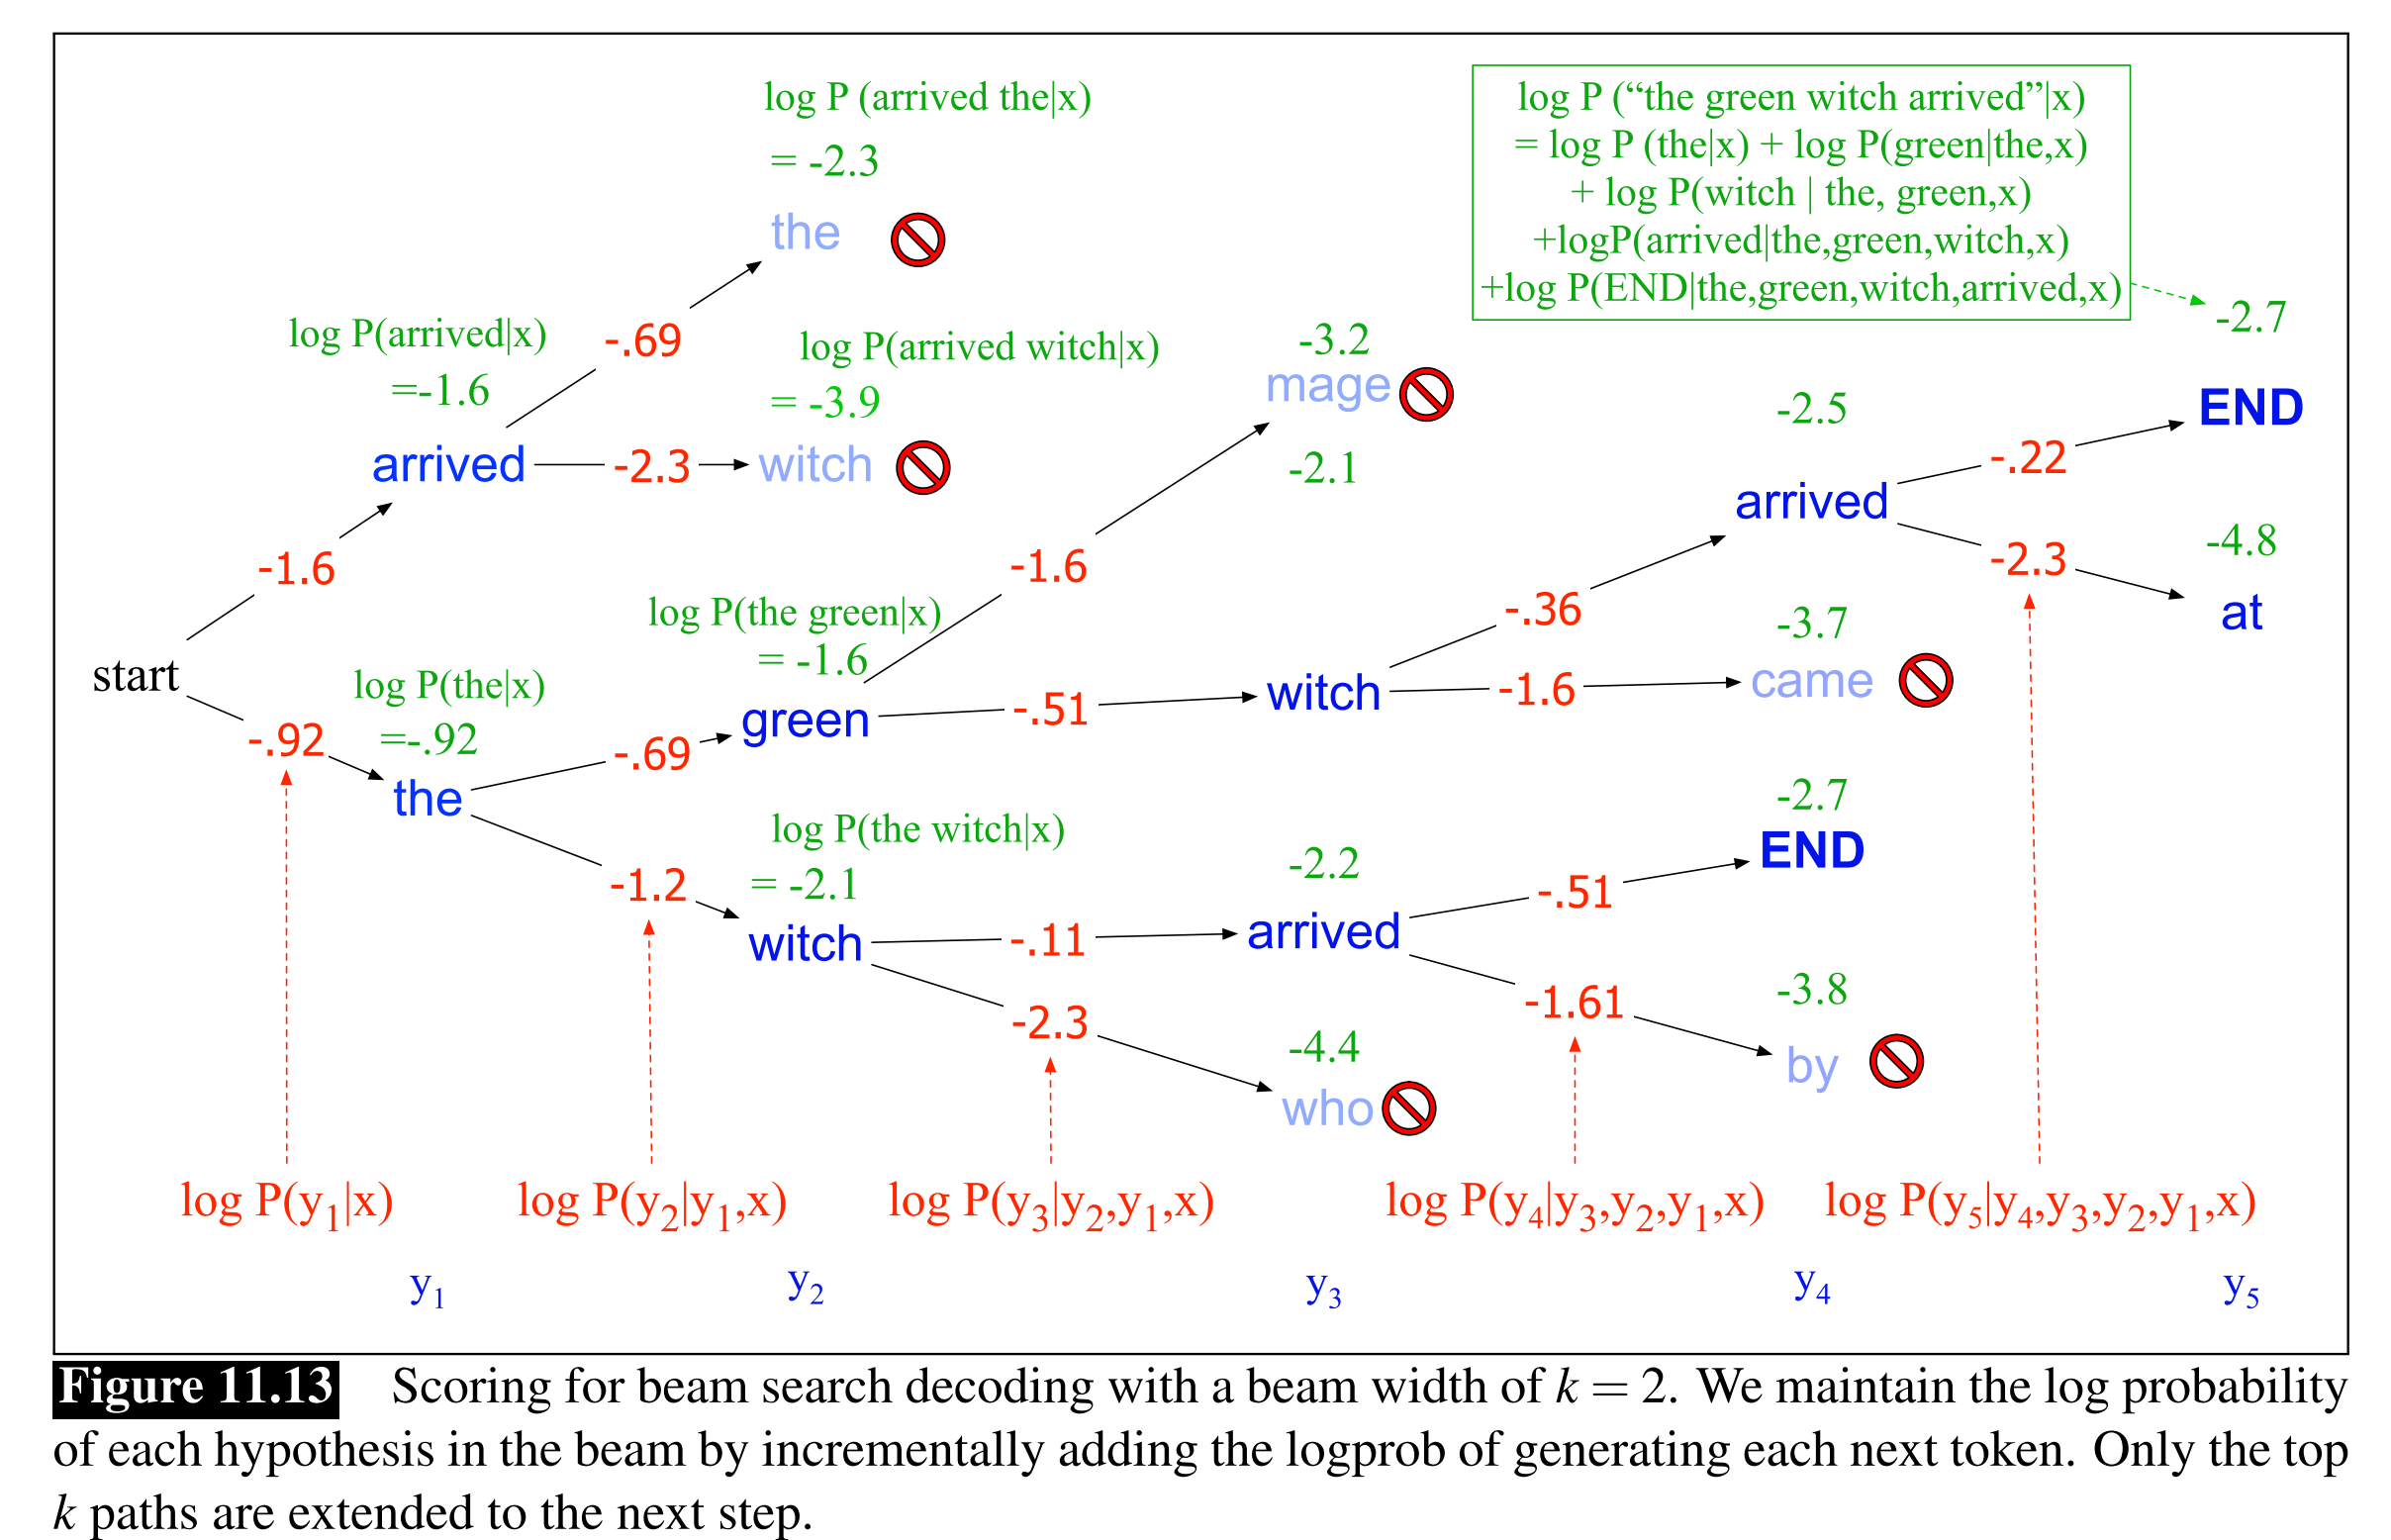
\includegraphics[width=\columnwidth]{img/beam1.png}
    \caption{An example of Beam Search.}
    \label{fig:entropy}
\end{figure}
\end{comment}

% Dan Jurafsky
% https://web.stanford.edu/~jurafsky/slp3/ed3book.pdf


%We summarize our contributions as follows:



% \acil{I recommend converting these to statements (indicating contributions of the paper) rather than questions for better effect. @Amitava sir, thoughts?}
%\end{strip}


